%%
%% This is file `sample-sigconf-authordraft.tex',
%% generated with the docstrip utility.
%%
%% The original source files were:
%%
%% samples.dtx  (with options: `all,proceedings,bibtex,authordraft')
%% 
%% IMPORTANT NOTICE:
%% 
%% For the copyright see the source file.
%% 
%% Any modified versions of this file must be renamed
%% with new filenames distinct from sample-sigconf-authordraft.tex.
%% 
%% For distribution of the original source see the terms
%% for copying and modification in the file samples.dtx.
%% 
%% This generated file may be distributed as long as the
%% original source files, as listed above, are part of the
%% same distribution. (The sources need not necessarily be
%% in the same archive or directory.)
%%
%%
%% Commands for TeXCount
%TC:macro \cite [option:text,text]
%TC:macro \citep [option:text,text]
%TC:macro \citet [option:text,text]
%TC:envir table 0 1
%TC:envir table* 0 1
%TC:envir tabular [ignore] word
%TC:envir displaymath 0 word
%TC:envir math 0 word
%TC:envir comment 0 0
%%
%% The first command in your LaTeX source must be the \documentclass
%% command.
%%
%% For submission and review of your manuscript please change the
%% command to \documentclass[manuscript, screen, review]{acmart}.
%%
%% When submitting camera ready or to TAPS, please change the command
%% to \documentclass[sigconf]{acmart} or whichever template is required
%% for your publication.
%%
%%
\documentclass[sigplan,10pt]{acmart}
%%
%% \BibTeX command to typeset BibTeX logo in the docs
\AtBeginDocument{%
  \providecommand\BibTeX{{%
    Bib\TeX}}}

%% Rights management information.  This information is sent to you
%% when you complete the rights form.  These commands have SAMPLE
%% values in them; it is your responsibility as an author to replace
%% the commands and values with those provided to you when you
%% complete the rights form.
\setcopyright{acmlicensed}
\copyrightyear{2018}
\acmYear{2018}
\acmDOI{XXXXXXX.XXXXXXX}
%% These commands are for a PROCEEDINGS abstract or paper.
\acmConference[Conference acronym 'XX]{Make sure to enter the correct
  conference title from your rights confirmation email}{June 03--05,
  2018}{Woodstock, NY}
%%
%%  Uncomment \acmBooktitle if the title of the proceedings is different
%%  from ``Proceedings of ...''!
%%
%%\acmBooktitle{Woodstock '18: ACM Symposium on Neural Gaze Detection,
%%  June 03--05, 2018, Woodstock, NY}
\acmISBN{978-1-4503-XXXX-X/2018/06}


%%
%% Submission ID.
%% Use this when submitting an article to a sponsored event. You'll
%% receive a unique submission ID from the organizers
%% of the event, and this ID should be used as the parameter to this command.
%%\acmSubmissionID{123-A56-BU3}

%%
%% For managing citations, it is recommended to use bibliography
%% files in BibTeX format.
%%
%% You can then either use BibTeX with the ACM-Reference-Format style,
%% or BibLaTeX with the acmnumeric or acmauthoryear sytles, that include
%% support for advanced citation of software artefact from the
%% biblatex-software package, also separately available on CTAN.
%%
%% Look at the sample-*-biblatex.tex files for templates showcasing
%% the biblatex styles.
%%

%%
%% The majority of ACM publications use numbered citations and
%% references.  The command \citestyle{authoryear} switches to the
%% "author year" style.
%%
%% If you are preparing content for an event
%% sponsored by ACM SIGGRAPH, you must use the "author year" style of
%% citations and references.
%% Uncommenting
%% the next command will enable that style.
%%\citestyle{acmauthoryear}

%\usepackage{todonotes}
\usepackage{booktabs}
\usepackage{multirow}
\usepackage{rotating}
 \usepackage{proof}
\usepackage{array}
\usepackage{iris}
\newcolumntype{O}[1]{>{\raggedright\arraybackslash}m{#1}}
\newcolumntype{P}[1]{>{\centering\arraybackslash}m{#1}}
\newcolumntype{Q}[1]{>{\raggedleft\arraybackslash}m{#1}}
\newcolumntype{S}{>{\centering\arraybackslash}m{2cm}}
% Useful macros from Isaac Oscar Gariano: a very simple library for author-specific change notations:
%  After calling \newAuthor{<name>}{<colour>}
% You can use \<name>{<text>} to add a comment
% Or \<name>A{<text>} to  write stuff in your colour (to denote additional text)
% Or \<name>B{<text>} is similar, but changes the background (to highlight stuff?)
% I may add more commands later
% (there's a 'changes' package with similar functionality, but it has a habit of breaking when you use it with  the Define environment)
\newcommand\newAuthor[2]{%
        \ExpandArgs{c}\newcommand{#1}[1]{\todo[color=#2!10, bordercolor=#2, inline]{\textbf{#1:}~##1}}
	\ExpandArgs{c}\newcommand{#1A}[1]{\textcolor{#2}{##1}}
        \ExpandArgs{c}\newcommand{#1B}[1]{\colorbox{#2!30}{\textcolor{black}{##1}}}}
\newtheorem*{remark}{Remark}
\newcommand{\loc}{\textsf{Loc}}
\newcommand{\sepimp}{\mathrel{-\mkern-6mu*}}
\newcommand{\blackdiamond}{\rotatebox[origin=c]{45}{$\vcenter{\hbox{$\scriptscriptstyle\blacksquare$}}$}}

\newAuthor{Ismail}{blue}
\newAuthor{Colin}{cyan}

%% The "title" command has an optional parameter,
\usepackage{amsthm}
\theoremstyle{definition}
\newtheorem{definition}{Definition}[section]
%%
%% end of the preamble, start of the body of the document source.
\begin{document}

%%
%% The "title" command has an optional parameter,
%% allowing the author to define a "short title" to be used in page headers.
\title{On Verification Patterns for Low-Level Systems via Modal Abstractions}

%%
%% The "author" command and its associated commands are used to define
%% the authors and their affiliations.
%% Of note is the shared affiliation of the first two authors, and the
%% "authornote" and "authornotemark" commands
%% used to denote shared contribution to the research.
% Commentout
\author{Ismail Kuru}
%\authornote{Both authors contributed equally to this research.}
\email{ik335@drexel.edu}
\orcid{0000-0002-5796-2150}
\affiliation{%
  \institution{Drexel University}
  \city{Philadelphia}
  \state{PA}
  \country{USA}
}
\author{Colin Gordon}
%\authornotemark[1]
\email{csg63@drexel.edu}
\orcid{0000-0002-9012-4490}
\affiliation{%
  \institution{Drexel University}
  \city{Philadelphia}
  \state{PA}
  \country{USA}
}

%%
%% By default, the full list of authors will be used in the page
%% headers. Often, this list is too long, and will overlap
%% other information printed in the page headers. This command allows
%% the author to define a more concise list
%% of authors' names for this purpose.
\renewcommand{\shortauthors}{}

%%
%% The abstract is a short summary of the work to be presented in the
%% article.
\begin{abstract}
  Although they differ in the functionality they offer, low-level systems exhibit certain patterns of design and utilization of computing resources.
  In this paper we examine how modalities have emerged as a common structure in formal verification
  of low-level software, and explain how many recent examples naturally share 
  common structure in the relationship between the modalities and software features they are used
  to reason about.
  We explain how the concept of a \emph{resource context} (a class of system resources
  to reason about) naturally corresponds to families of modal operators indexed by
  system data, and how this naturally leads to using modal assertions to describe
  \emph{resource elements} (data in the relevant context).
  We also describe extensions of this idea to ongoing work in formal verification
  of filesystems code.
  % \todo[inline,color=cyan]{Ismail, why did you comment out my suggestion and keep the original?}
  % \todo[inline,color=pink]{Sorry, I thought I did the other way}
\end{abstract}

%%
%% The code below is generated by the tool at http://dl.acm.org/ccs.cfm.
%% Please copy and paste the code instead of the example below.
%%
%\begin{CCSXML}
%<ccs2012>
% <concept>
%  <concept_id>00000000.0000000.0000000</concept_id>
%  <concept_desc>Do Not Use This Code, Generate the Correct Terms for Your Paper</concept_desc>
%  <concept_significance>500</concept_significance>
% </concept>
% <concept>
%  <concept_id>00000000.00000000.00000000</concept_id>
%  <concept_desc>Do Not Use This Code, Generate the Correct Terms for Your Paper</concept_desc>
%  <concept_significance>300</concept_significance>
% </concept>
% <concept>
%  <concept_id>00000000.00000000.00000000</concept_id>
%  <concept_desc>Do Not Use This Code, Generate the Correct Terms for Your Paper</concept_desc>
%  <concept_significance>100</concept_significance>
% </concept>
% <concept>
%  <concept_id>00000000.00000000.00000000</concept_id>
%  <concept_desc>Do Not Use This Code, Generate the Correct Terms for Your Paper</concept_desc>
%  <concept_significance>100</concept_significance>
% </concept>
%</ccs2012>
%\end{CCSXML}
%
%\ccsdesc[500]{Do Not Use This Code~Generate the Correct Terms for Your Paper}
%\ccsdesc[300]{Do Not Use This Code~Generate the Correct Terms for Your Paper}
%\ccsdesc{Do Not Use This Code~Generate the Correct Terms for Your Paper}
%\ccsdesc[100]{Do Not Use This Code~Generate the Correct Terms for Your Paper}
%
%%%
%%% Keywords. The author(s) should pick words that accurately describe
%%% the work being presented. Separate the keywords with commas.
%\keywords{Do, Not, Us, This, Code, Put, the, Correct, Terms, for, Your, Paper}
%% A "teaser" image appears between the author and affiliation
%% information and the body of the document, and typically spans the
%% page.
%\begin{teaserfigure}
%  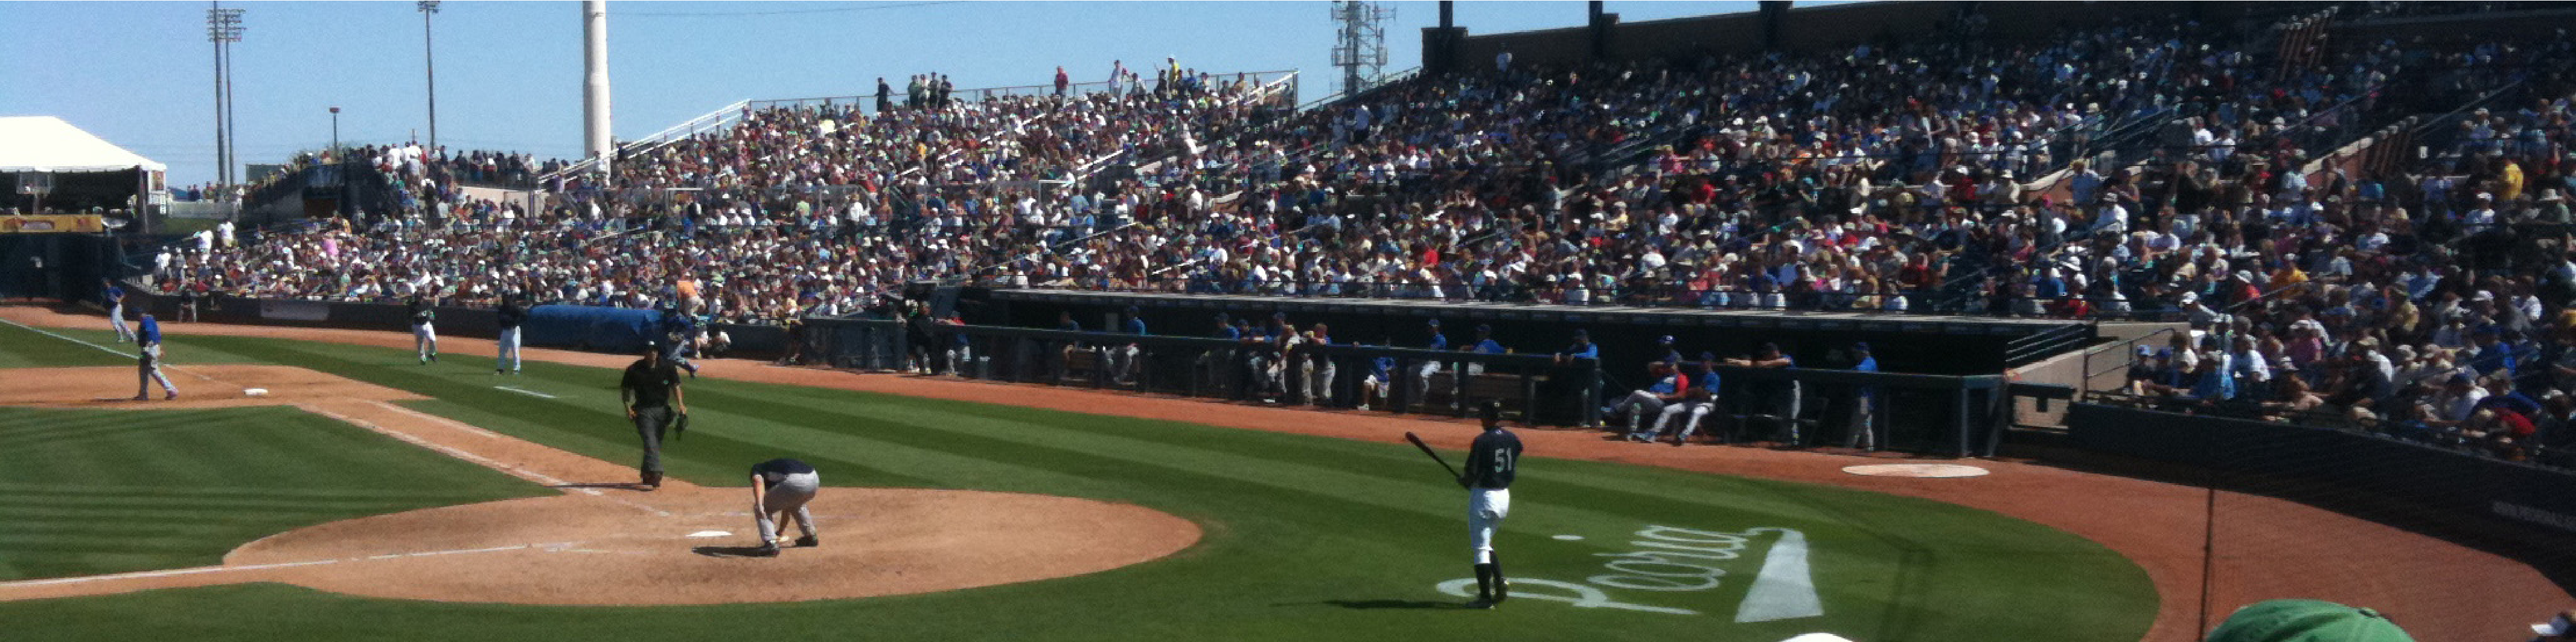
\includegraphics[width=\textwidth]{sampleteaser}
%  \caption{Seattle Mariners at Spring Training, 2010.}
%  \Description{Enjoying the baseball game from the third-base
%  seats. Ichiro Suzuki preparing to bat.}
%  \label{fig:teaser}
%\end{teaserfigure}

%\received{20 February 2007}
%\received[revised]{12 March 2009}
%\received[accepted]{5 June 2009}

%%
%% This command processes the author and affiliation and title
%% information and builds the first part of the formatted document.
\maketitle
\section{Introduction}
Although they differ in the functionality they offer, low-level systems exhibit certain patterns of design and utilization of computing resources.
Systems software, in general, interfaces with an underlying computing substrate such that any software system at any higher level in the software stack can (at least indirectly) utilize the resources of the machine.
The last layer of software before the hardware is naturally critical to the correctness of an overall system,
as essentially all software built on top of it assumes its correctness.
%Assuming verified hardware, this makes the correctness of the system software critical to the rest of the software stack. 
%Because they interface with the hardware, abstractions and their implementations are intricate and error-prone. 
And because hardware is complex and highly diverse, the implementation of those lowest layers
of the software stack is typically intricate and naturally error-prone, despite how critical its correctness is.
Typically systems software has, as a primary focus, the task of \emph{abstracting} from hardware details to simplify 
the construction of higher layers of the stack.

% \subsection{Conclusion \& Contributions}
% \paragraph{Conclusion} 
Interacting with computing resources is the essential point which shapes the design of low-level systems software. 
Exploiting these design choices has been an important field of study.
This survey examines these common patterns in systems software, and their relationships
to modalities. We believe that certain properties of modalities enable us to understand and 
address the verification challenges of these systems by tailoring specification and proof
to the same patterns used to design the systems.

\textit{Contributions} We argue that modal abstractions can be used to identify and abstract system verification challenges. We justify our perspective by discussing prior systems that have successfully used modalities for system verification, arguing that they fit into the verification design pattern we articulate, and explaining how this approach might apply to other systems' verification challenges.
\begin{itemize}
\item \textbf{Identifying System Verification Challenges}: We start with identifying common patterns in system verification: \emph{virtualization, sharing, and translation}.
\item \textbf{Introducing Modal \emph{Resource Contexts}}: Then we discuss the concept of \emph{resource} which has already been an essential concept in the design of systems. Inspired by the concept of resource in the systems, we define what a resource and its context are in the modal abstractions.
\item \textbf{Introducing \emph{Nominals for System Resources}}:
Existing logics for systems software must frequently identify
individual resources within a given context ---
nominalization (in the sense of hybrid logic) enables identifying a resource in its context. 
For example, a filesystem transaction is a context of resources for in-memory updated disk blocks
which have not yet been saved to disk.
The transaction identifier is used to associate a transaction with a disk-block to be persisted so that, 
in case of a crash while persisting updated disk-blocks, the filesystem can rollback the 
\emph{already persisted} disk-blocks of the transaction, and reach to the previous consistent disk state. 
We discuss other examples to contextualize the existing systems surveyed.
% to be able to do so, both the updated in-memory disk blocks and the transaction must refer to the transaction 
% identifier -- \emph{strong nominalization}. 
% in another example, virtual memory references (resources) in 
% an address space (resource context), which can be uniquely identified with a root address (the nominal) 
% of its page-table tree, are \emph{agnostic} to the address space that they are in. 
% However, they can only be accessed (be valid) in the address space to which they are agnostic. 
% However, then an address space switch happens, the virtual memory references of the previous address 
% space must be made inaccessible. To be able to do so, although virtual memory references do not hold any 
% piece of information related to their address space, we still have to associate them. 
% We call this kind of unilateral nominalization -- \emph{weak nominalization}.
% \todo[inline,color=cyan]{I left this paragraph alone, mostly, but it's too detailed for the new intro section position here}
\item \textbf{Taxonomy of Current Modal Approaches in System Verification}: Based on these concepts defined, we summarize contemporary verification efforts using modal abstractions. We choose them from different domains, for example, reasoning about weak memory models and storage persistence ~\cite{tejthesis,perennialgit,tejperennial19,larsnextgen25,fsl,fsl++,derekrustbelt20,kuru2025modalabstractionsvirtualizingmemory,amalreal2024} because we would like to justify that our \emph{definitions} are not domain dependent.
\end{itemize}


\section{Background on Modal Logics for Programs, and Low-Level Systems Software}

This section briefly recalls related concepts from modal logic of particular relevance
to our taxonomy, which should be familiar but benefit from fixing notation (Section \ref{sec:modalbackground}),
and enough general background on the systems software concepts organized by our taxonomy
for the connections to modalities to be clear (Section \ref{sec:background}).

\subsection{Hybrid Logic, Dynamic Logic, and Nominals in Program Logics}
\label{sec:modalbackground}
\textit{Dynamic Logics as Program Logics}
We believe that for the kinds of informal reasoning and the sorts of data structures discussed in the previous section, ideas from modal logic are a promising approach to formalization and verification.
Broadly speaking, modal logics incorporate \emph{modal operators}, which take as arguments a proposition expected to be true in another time~\cite{pnueli1977temporal}, place~\cite{gordon2019modal,goranko1996hierarchies,areces2001hybrid,gargov1993modal,murphy2004symmetric}, circumstance or point-of-view~\cite{hintikka1962knowledge,halpern1985guide}, and result in a proposition true in the \emph{current} time, place, or circumstance at which the truth of the use of the modal operator is being evaluated. Classic examples include modal necessity $\square P$ describing that $P$ is \emph{necessarily} true, $\mathsf{G}~P$ meaning $P$ is true \emph{globally} (i.e., forever from this time onwards in temporal logics), or $K_i(P)$ describing that a particular participant $i$ \emph{knows} that $P$ is true. The latter is an example of \emph{multimodal} logic, where there is an family of modalities (modal operators) parameterized by some dimension of interest (there, participants).

\emph{Dynamic logic}~\cite{pratt1976semantical} is a (multi)modal logic of weakest preconditions~\cite{dijkstra-75} which works with modalities of the form $[p](P)$, which states that \emph{in the current program state}, \emph{if} program $p$ is run then afterwards $P$ will hold (modulo non-termination).
This same idea is used to encode Hoare triples in the Iris program logic~\cite{jung2018iris}, using the same encoding as in Pratt's original presentation, where a Hoare triple $\{P\}C\{Q\}$ is encoded as $P\rightarrow[C](Q)$.
Iris is now one of the most successful foundational program logics, and its rich support for
extending the base logic with additional modalities~\cite{krebbers2017essence} means that
modal logics, and in particular dynamic logic, now play an outsized role in program verification ---
many challenging proofs of program correctness use a substructural dynamic logic containing
many additional modalities which interact with the weakest precondition modality.

% A hallmark of a unary logical operator $M$ being a modality is if $M$ satisfies a property akin to $(\varphi\rightarrow\psi)\rightarrow M(\varphi)\rightarrow M(\psi)$, which roughly states that modus ponens holds under the modality.\footnote{Afficionados of modal logic will note that this property is not quite Axiom K (which requires the initial implication to also hold under $M$), but follows from K and a necessitation rule $\varphi\rightarrow M(\varphi)$. Non-necessitive modalities typically satisfy the weaker property we call out above.} This and related laws allow transporting general reasoning into the specific contexts or hypotheticals modeled by the modalities.

\textit{Hybrid Logic} Hybrid logics~\cite{blackburn1995hybrid,goranko1996hierarchies,gargov1993modal,areces2001hybrid,brauner2010hybrid} are a class of modal logics that add two primary new concepts to a logic. Nominals $\ell \in \textsf{Loc}$ uniquely identify points in a model (e.g., a particular state), so there is exactly one point in the model where a nominal $\loc$ is true. Satisfaction operators are modal operators indexed by nominals, which enable claims about the truth of another proposition at some arbitrary point in the model identified by a nominal. Traditionally $@_l\varphi$ asserts that $\varphi$ is true in the state identified by $l$. Conceptually, given our context, we might like $l$ to indicate truth in a particular data structure $l$.  However, most prior work on hybrid logics works in classical logics rather than a substructural setting like separation logic. 
Newer work ~\cite{tejthesis,perennialgit,tejperennial19,larsnextgen25,fsl,fsl++,derekrustbelt20,kuru2025modalabstractionsvirtualizingmemory,amalreal2024}  surveyed here adapts this idea to deal with different structures specified in
separation logic.
%We adapt these ideas to assertions of the form $@[l]\varphi$ asserts that $\varphi$ is true in a data structure with \emph{logical} state $\sigma$ \emph{at location} $l$.
% In practice we must design variants of this for each kind of structure we wish to apply this to, e.g. tree nodes, free list, or snapshots.
%This section provides details of and models for each modal abstraction, focusing on how each data structure can act as a model for a data-structure-specific logic.
%We continue to motivate the development with aspects of the write amplification process described in the previous section; Section \ref{sec:evaluation} provides further examples using the modal abstractions in proofs.
% \paragraph{Temporal Operators}
% The best known class of modal logics in the systems community is undoubtedly temporal logics (whether \textsc{LTL}~\cite{pnueli1977temporal}, \textsc{CTL}~\cite{emerson1982using}, \textsc{TLA}~\cite{lamport1994temporal}, or others),
% due in part to Lamport's influence~\cite{lamport2002specifying} leading to its not-infrequent use in specifying
% distributed algorithms \cite{ongaro2014search,ailijiang2019wpaxos}.

\textit{Nominalization}
Some classes of assertions benefit specifically from \emph{naming} the explicit conditions where they are true (as opposed to simply requiring them to be true \emph{somewhere} or \emph{everywhere} as in the most classic modal operators).
% This naming generally resembles
% the \emph{satisfaction} operator of 
% \emph{hybrid logic}~\cite{blackburn1995hybrid,areces2001hybrid}: $@_\iota P$ which evaluates the truth of $P$ at the named (Kripke model) state $\iota$. 
Because these named conditions strongly resemble the nominals of hybrid logic,
we refer to the general idea of naming circumstances explicitly as \emph{nominalization},
even though not all of the examples we discuss are actually hybrid logics.

An example use of state naming explicitly in the assertion appears in program logics 
with usage protocols (e.g. state transition systems resembling typestate~\cite{strom1986typestate,garcia2014foundations}, which ensure
the operations applied to some data occur in a specified order, and that invariants for various conceptual states of the data
--- such as a file being open or closed --- are respected). 
Protocol assertions are \emph{annotated with the name of the last (abstract) state at which the protocol is ensured}.
A classic application of this idea to systems is 
Halpern et al.'s work adapting modal logics of
knowledge to deal with distributed systems~\cite{halpern1990knowledge,halpern1989modelling,halpern2017reasoning}.
In most of that line of work, $\mathcal{K}_a(P)$ indicates that the node $a$ in the system \emph{knows} or \emph{possesses knowledge of} $P$
(for example, a Raft node may ``know'' a lower bound on the commit index).
Alternatively, a modality $@_i(P)$ may represent that $P$ is true of/at the specific node $i$~\cite{gordon2019modal} (e.g., that node $i$ has stored a certain
piece of data to reliable storage).
These permit capturing specific concepts relevant to the correctness (and reasoning about correctness) of a certain class of systems,
involving facts about specific named entities in the system.

In each of these cases, the fact that these facts are described using modalities with the core modal property $P \Rightarrow Q$, then $M(P) \Rightarrow M(Q)$ means, for example, that if a
process $p$ knows that the commit index is greater than 5 (e.g., $\mathcal{K}_p(\mathsf{commitIndex} > 5)$)
no extra work is required to conclude that the node knows it is greater than 3 (i.e., that $\mathcal{K}_p(\mathsf{commitIndex} > 3)$),
because this follows from standard properties of modal operators as described above.
In contrast, if verification instead used a custom assertion $\mathsf{minCommitIndex}(5)$ to represent the former knowledge,
one would need to separately provide custom reasoning to conclude $\mathsf{minCommitIndex}(3)$.
As our survey shows, the value of the modal view (which grants both intuitive specifications and natural
reasoning principles) is becoming apparent in systems software verification.

\subsection{Virtualization in Systems Software}
\label{sec:background}
One of the most common forms of abstraction provided by systems software is \emph{virtualization},
which abstracts the relationship between conceptual and physical computing resources.
Upper-levels of the software stack work with these conceptual --- \emph{virtual} ---
resources, while the lower levels of systems software deal with the translation
of requests expressed in terms of virtual resources into operations on physical resources.

Operating System (OS) kernels virtualize memory locations and quantity (via virtual memory and paging~\cite{Denning1970VM}).
Distributed language runtimes may virtualize addresses, even when processes may migrate across machines~\cite{jul1988fine}.
Filesystems virtualize locations on disk~\cite{rodeh2013btrfs,hitz1994file,Rosenblum1992LFS,bonwick2003zettabyte}.
Programs built on top of the corresponding systems software layer work logically at the level of these virtualized resources,
and it makes sense to specify the systems software directly in terms of those abstractions.

\textit{Access by Translation}
Accessing virtualized resources via translation is a common way to virtualize notions of location (e.g.,
virtual memory addresses, inodes or object IDs instead of disk addresses~\cite{bonwick2003zettabyte,hitz1994file,Rosenblum1992LFS,rodeh2013btrfs}).
%Accessing the hardware resources in the presence of sharing means having more resource references (references to the virtualized resources) to access the \emph{mapped} resources that are physical and potentially fewer. 
B-trees, page tables, and related structures both behave like maps, when the corresponding physical resources exist as such
just in a different location.
Control over the lookup process (e.g, handling the case of a missing translation entry) allows for additional flexibility,
such as filling holes in sparse files, or demand paging (both from disk or lazily populating anonymous initially-zeroed mappings).
Although the realization of these maps may differ from system to system based on the context (and sometimes hardware details),
they are semantically --- logically --- partial maps, worth treating as such in verification.

\subsubsection{Virtualization of Memory Locations}
\label{sec:backgroundonmachinemodel}
A typical general purpose computer virtualizes  memory resources in RAM.
A program asking for a memory unit from an operating system kernel is served with a memory address that is \emph{virtualized}
such that it may be \emph{mapped to} a physical RAM location or not. 
As our informal definition suggests, the common technique for \emph{virtualization} of memory locations in OS 
kernels relies \emph{translating} (\emph{mapping}) virtual addresses into physical ones. 
The conceptual address-translation map is implemented with processor's page-table trees. A virtual address indexing into the different levels of the page-table tree 
are blocks of memory which serve as nodes of the tree along a particular lookup path. 
Fabrication of virtual addresses out of limited physical addresses is provided with entries 
in the page-table tree where each points to a physical address aligned to 4KB (4096 byte) boundaries. 
An address translation requires traversal of a series of tables starting from top level, and it is  conventionally referred as a \emph{page-table walk}. 
The traversal ends in the level 1 page table with the final lookup to the actual page of physical memory holding the requested data, and the low-order 12 bits being used to index into this page.
%\begin{figure}
%    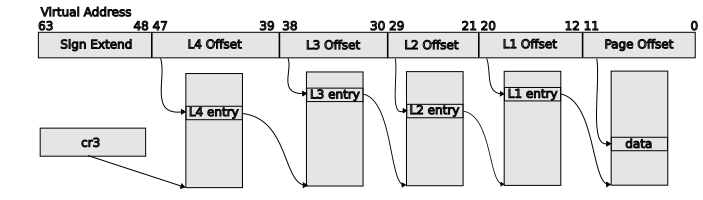
\includegraphics[width=\columnwidth]{pagetables2.png}
%    \caption{x86-64 page table lookups.}
%    \label{fig:pagetables}
%\end{figure}

A page table tree is referred to as a (virtual) \emph{address space}, as it presents an abstraction
of how different memory addresses could be related in space.
This functionality is used by operating systems to present fictional collocation or separation of resources:
a range of logically (virtually) contiguous memory addresses may be translated to a range of physically disparate locations
in actual memory.
The address space then acts as a kind of container for virtualized memory resources tied to that container.

% \paragraph{Virtual Memory Managers(VMM) with Multiple Address-Spaces}
% \label{sec:backgroundonvmm}
% \todo{change the text}
% An intuition for the abstraction that \emph{contains} a page-table tree is called an \emph{address-space} of a process whose virtual addresses to physical addresses. 
A typical OS manages multiple address spaces at once.
Each program is associated with a unique page table tree, which is stored in a specific hardware register (e.g., \texttt{cr3}). 
Using different mappings, which map only disjoint portions of physical memory in the map's codomain, 
is how the OS ensures memory isolation between processes. 


\subsubsection{Virtualized Resources in Filesystems}
Another important computer resource computer resource that is \emph{virtualized} for access is disk blocks. 
Filesystems are software components that abstract disk access on behalf of normal programs.
Similarly to how VMMs use page-table trees to fabricate more memory addresses than actually exist, filesystems use indexing maps to fabricate more virtual disk-page addresses (which are conventionally called disk-pages) to be distinguished from physical disk-block addresses.
When a regular program accesses a file, it requests a specific logical offset from the start of that file's contents.
As with virtual memory, the filesystem may map adjacent logical blocks of a single file to physically disparate parts of the disk (or even
to different disks), though this translation mapping is implemented entirely in software (as opposed to the hardware cooperation that exists
for memory virtualization).

% \paragraph{Overview of Policies in Filesystems}
Filesystems not only handle the address-translation from a disk-page to a disk-block but also need to handle different modes of computing, representing where to find disk resources: a disk block may live on a disk in stable storage,
or the most up-to-date version of a block may live only in memory (for the filesystem to write to disk at a later time, batched for efficiency).
To handle the consistency of the disk resources in the existence of different modes of execution, filesystems employ different policies when indexing the disk resource.
Which data-structure is going to be used to implement address-translation from disk-pages to disk-blocks? 
What is going to be the \emph{update-policy} to the indexing map implementing address-translation which defines the \emph{consistency-policy} for the disk resources? 
Different filesystem implementations give different answers to these questions. 

% One example answer to updating policy is copy-on-write (\textsf{CoW}). A (\textsf{CoW}) filesystem performs updates by copying modified data to \emph{new and unused} locations on disk rather than updating \emph{in-place}, ensuring that in the absence of physical storage corruption, there is \emph{always} a fully consistent filesystem on disk, removing the need for recovery from journals in the case of a crash, which can be very expensive for large volumes.

%\textsf{ModFS} is implemented in \textsc{Go}~\cite{donovan2015go}, using the FUSE~\cite{fuse} interface to run a filesystem in usermode. \textsf{ModFS}'s code is translated to \textsf{Roqc} using the \textsf{Goose}~\cite{chajed2019verifying,chajed2021gojournal} tool, which translates a significant subset of \textsf{Go} to \textsf{Roqc} to permit formal verification of \textsc{Go} code using \textsf{Iris}~\cite{jung2018iris}. \textsf{Goose} generates code in an extension of \textsf{Iris}'s \textsf{HeapLang} with libraries for disk manipulation and \textsc{Go} primitive types (e.g., maps) as shown in Figure \ref{fig:modfslayout}.

%On the left part of Figure \ref{fig:modfslayout}, we see the shaded region -- \textsf{ModFs} storage layer-- under the yellow layer --- the \textsf{ModFs} system call layer. 
%We have verified the parts of the shaded storage layer involved in creating a new on-disk snapshot, up to an axiomatized specification of of the \textsf{Bcache} component that implements a simple in-memory cache of disk blocks.
%This primarily involves the \textbf{write\_amplification} function on btree nodes (from the \textsf{Btree} module), and its associated dependencies, including the \textbf{split}, \textbf{put}, and \textbf{del}(ete) operations on nodes, and the \textbf{write} serialization function.
%This also includes snapshot operations including \textbf{snap\_initialize} and \textbf{snap\_alloc} functions (among others) in the \textsf{Snapshot} module, and freelist operations (\textbf{free} and \textbf{allocate}) from \textsf{Freelist}, as well as the supporting functions from the \textsf{Chunk} (roughly a structured disk block abstraction), \textsf{PageMap} (raw disk block abstraction), \textsf{and Lock} (thread synchronization via a global lock map) modules.
%\textsf{Storage} (a data structure of runtime pointers\colinsays{doesn't really explain it, I don't know what this component is/does}), \textsf{BtrItr} (an iterator library), \textsf{inode}, and \textsf{Btree} have not yet been fully verified, though the components involved in write amplification have been verified. The filesystem does run and standard filesystem functionality (core file and directory operations) work.
%This paper focuses on the verification of write amplification, which is verified up to a small number of axioms for \textsf{Go} data structures\colinsays{update w/ very short summary of remaining admits} and the unverified \textsf{Bcache} specification.
%\colinsaysinl{How many lines of code are covered by the verification? (excluding the bcache) This might help assuage reviewer concerns that we're not done, by making the scope of this project more explicit so ``why didn't you finish'' has a self-evident answer of ``because they already did a ton of work''}

%\textsf{ModFs} is a \textsf{CoW} file system where the mapping of the logical locations, e.g., file pages indexed by file offsets, to disk locations by employing a \textsf{CoW} tree \cite{Astrahan1976SystemR,shadowclone} structure. In Figure \ref{fig:cow_index_tree}, we see that accessing and updating the $\textsf{page}_n$ of file \textsf{"foo"} referred by the file offset $\textsf{offset}$ 
%\[ \textsf{write}(\textit{foo},\textsf{offset})\]
%requires locating the corresponding physical disk block of the in-memory $\textsf{page}_n$ whose mapping is establised the \textit{copy-on-write} index tree (in the middle layer). Like Btrfs ~\cite{}, \textsf{ModFs} indexes all filesystem objects (e.g. files and directories) as a nested trees, and to map a logical page to a physical page, the file system first locates the root of the nested index-tree belonging to \textsf{"foo"}.

% \paragraph{An Example to a Policy for Updating Disk Index Tree}
% \todo[inline,color=cyan]{This gets too detailed, and is talking about the details of ModFS itself. 
% If we're casting this
% as a survey, we probably don't want to talk about ModFS except in passing (like towards the end of the paper), but want to focus on things that are at least publicly available.
% This level of detail is also way more than later parts of the paper require for understanding --- generally
% we only want a background section to cover enough for the later parts of the paper to make sense. Any
% extra depth just ends up burning reader patience.}
% Semantically, in \textsf{ModFS}~\cite{} (as in other \textsf{CoW} filesystems~\cite{young1992episode,bonwick2003zettabyte,rodeh2013btrfs,Rosenblum1992LFS,hitz1994file}) any update to file data or metadata is realized on  unused disk locations by treating the tree as a persistent data structure. 
% As an example, Figure \ref{fig:cowindex} shows that an update to the file $\textsf{"foo"}$ at $\textsf{"offset"}$ ends up with locating the related disk chunk(multiple disk-pages) in the gray region, copying it to newly allocated disk chunks (dotted chunks on the right side of the bold long-dash-point line of the middle layer withing dotted section), and performing the update on these newly-allocated disk blocks. This requires further updates to those metadata blocks which previously referred to the old block locations to instead reference the newly-allocated blocks. This must be repeated until the allocation/update of the new chunks percolates up to the root (including the root), through a process called \textsf{\textit{write-amplification}}.

% \begin{figure}[t]
%     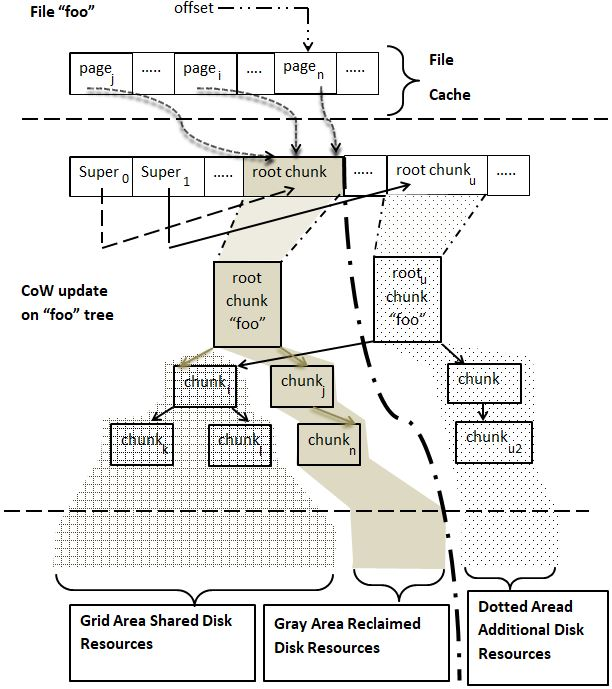
\includegraphics[width=0.75\columnwidth]{cow_index.png}
%     \caption{A Filesystem called \textsf{Modfs} Indexing its Physical Pages for File Pages with CoW (copy-on-write) Tree}
%     \label{fig:cowindex}
% \end{figure}
% \paragraph{Examples to Different Policies on Navigating on Consistent Views of Disk}
% Like VMMs navigating between different address-spaces, a \textsf{CoW} filesystem switches from either the old to the new root yields consistent views of the filesystem at different points in time, each commonly referred to as a \emph{snapshot}. A \textsf{CoW} filesystems treat the snapshot abstraction as VMMs treat the address-space abstraction, container of the relevant resources. Like VMMs loading a process's memory mappings to be the current view of the memory by setting the control register to show the unique root address of the page-table tree of the process, the filesystem to atomically switch between consistent on-disk states, by updating the oldest so-called \emph{super} chunk at a fixed location on disk. Super chunks, as we see in Figure \ref{fig:cowindex} as ($\textsf{Super}_0$ and $\textsf{Super}_1$), are the first two blocks of the disk dedicated to keep the state of the file system which is composed of some meta-data on the filesystem, and most importantly to the root chunk of the filesystem index tree. 
% \begin{figure}
%     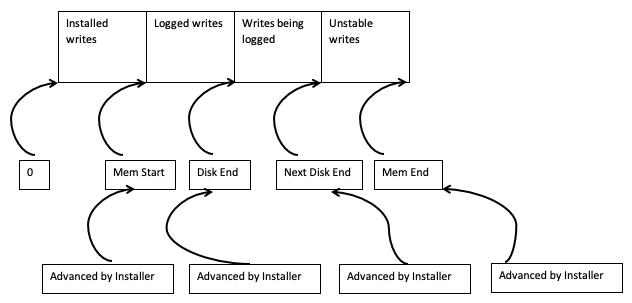
\includegraphics[width=\columnwidth]{journalling.png}
%     \caption{A Filesystem Utilizing \emph{Journalling} for Consistent Disk-Layout ~\cite{chajed2021gojournal}}
%     \label{fig:journal}
% \end{figure}
% \todo[inline,color=cyan]{This looks like it's verbatim copy-pasted from the ModFS draft; if this exact text
%   it used in this publication, it means we'd need to completely rewrite the relevant text in that draft.}
% Therefore, in case of a crash during the update to the \textsf{file "foo"}, we can reboot the file system from the previous persisted root, \textsf{root chunk}, via reading the $\textsf{Super}_0$. This means the whole disk consistency checks are unnecessary when recovering from a crash~\cite{bonwick2003zettabyte,hitz1994file}; recovery is immediate, as opposed to requiring hours or days~\cite{henson2006reducing,agrawal2009speedy} (or longer~\cite{henson2006chunkfs}) for recovering a large volume’s consistency from logs. 
% An important additional subtlety with this kind of filesystem is \emph{when} blocks in the reclaimed region can actually be reused: only \emph{after} the snapshot that made those blocks ``free'' has been completely written to disk. Allowing reuse before this could result in in-place updates: part of the new snapshot could attempt to store data in space used by the prior snapshot, allowing inconsistent on-disk structures.

While exceptions exist~\cite{bonwick2003zettabyte,rodeh2013btrfs,Rosenblum1992LFS,hitz1994file},
most filesystems will continue to store a given block of a given file in the same physical disk block for as long as the file exists.
These filesystems with in-place updates need to implement some form of \emph{journalling}~\cite{hagmann1987reimplementing,chutani1992episode} to ensure that a crash partway through an in-place update
can be rolled back using an undo journal that records the original contents before in-place modification (so original contents could be restored after a crash) 
or completed using a write-ahead journal that first writes new data in unused space before \emph{also} updating in place (so the journal entries could be re-applied after a crash). 
% \hrule
% In other words, unlike our ability to distinguish all resources (disk-pages and dis-kblocks) either being consistent under a snapshot or not in filesystems with \textsf{CoW}, with in-place updates, journalling mechanism does not allow such a claim. In other words, as we see in Figure \ref{fig:journal}, unlike \textsf{CoW}'s uniform persistency claim over disk resources under a snapshot as a resource container, elaborative bookkeeping mechanism of journalling leaves the filesystem treat disk resources in one of the resource groups in non-uniform fashion: disk-pages loaded into memory, updated disk-page not logged yet, updated and being logged or already logged disk-pages. Being able to treat the resources in a uniform fashion determines wwhether we need to consider the specification and proof of crash condition separately; instead a global never-violated invariant (not even temporarily broken) of the filesystem ensures the on-disk state is always consistent.
Because disk blocks associated with a file could now be in many states (on-disk, journaled but not updated in place, or both)
the specification of these systems is complex. And because some states are only possible after a system failure,
each line of filesystem code has two conceptual post-conditions: one for continued execution, and one for the stable
state established in the event of a hardware failure immediately after that operation.

\subsubsection{Reference-Counting Memory Reclamation}
In a typical configuration, allocating, deallocating and referencing memory locations for client code 
leaves the memory layout \emph{ideally} in a form of DAG (directed acyclic graph) with a unique root, which resembles the first stack pointer referencing the allocated memory. DAG abstraction instead of recursive descent tree allows non-duplication on the reference counts for the identical memory objects.
% To ease picturing the memory layout after a set of requests from the client code (for allocation, referencing etc.), we can think of the unique roots of DAGs as 
% \emph{super} block addresses -- this time multiple ones, not only two -- in Figure \ref{fig:cowindex}, 
% from which a path is created for a stack pointer reference to the allocated memory. 
%\todo[inline,color=cyan]{
%Why is this a DAG? Normally programs can easily create cycles, so the DAG bit requires a little more explanation.
%Do we mean that it is ``often'' the case that it's a DAG?}

It is safe to reclaim memory (for later reuse) when that memory allocation will no longer be used by the client program.
Since that property itself is undecidable, sound heuristics are used instead.
A common proxy for the program never accessing an allocation again is to check that there is no
access path from data a program can trivially access (e.g., local variables stored on the stack)
to a memory allocation --- that is, when the allocation is no longer \emph{reachable}.
In that case the program \emph{cannot} access the memory again, so the memory location can be reclaimed \emph{soundly} ---
i.e., without violating any access through a reference to it.

To reclaim the allocated memory location that is no longer being accessed, many systems use a well-known method called \emph{reference-counting} in which 
each memory allocation includes not only its data but also a counter of how many pointers to that memory exist in the rest of the program.
Any time a new reference to the allocated memory is created, the  counter is incremented,
and every time an existing reference is destroyed (by overwriting or dropping) the counter is decremented.\footnote{This may be done
using library functions for a reference counting system, or the operations may be inserted by a compiler.}
These reference counts are a sound (but incomplete) way to approximate reachability: if a decrement of a reference count
decrements the count to 0, no other references to that memory exist in the program, and the memory can be reclaimed.

Reasoning about the correctness of such code requires reasoning about these reachability relations and reference counts, relative to specific
stack frames.


% \paragraph{Buffering} Buffering is a technique used in variety of systems (filesystem page caching, write buffer in multi-processor architectures, 
% translation-lookaside-buffers for translated addresses etc.) to delay the costly operation (committing file pages, flushing buffered writes from write-cache 
% to memory etc.) making updates consistent.
% \paragraph{Consistency of Reads of Buffered Writes} Consistency of reads of any value potentially buffered depends on the semantics of 
% the operation making them \emph{observable}. A typical architecture such as Intel-x86 considers the \emph{flush} of buffered writes 
% \emph{non-deterministically} --- i.e., at any time at any number of buffered writes. On the other hand, a typical filesystem can follow a certain 
% policy to commit the in-memory file pages to the disk.   

\subsubsection{Weak Memory Models}
% I reworked this to be less general, and more about just weak memory, as thats all the survey section discusses.
Multi-core and multi-processor systems do not directly write every memory update back to memory (or even a coherent hardware cache)
individually, as this would be extremely slow. Instead, they effectively buffer reads and writes to and from memory
locally within each CPU core~\cite{owens2009better}\footnote{This is a layer below the better-known L1 cache, which is coherent across all CPUs in the system.}
so that operations can be partially reordered and batched to improve performance. For most code --- where the different CPUs are doing
independent work --- this is transparent to software. But fine-grained concurrent systems code which has multiple CPU cores
simultaneously coordinating access to shared memory must reason about these (effective) bufferings and reorderings, whose details vary
across CPU architectures.

Most of this coordination comes through reasoning about what \emph{will be true after local operations are published to memory},
or what \emph{will be true after remote operations become visible locally}~\cite{sieczkowski2015separation,dang2022compass,fsl}. Each of these flavors of contingent reasoning
depend on use of certain \emph{fence} or \emph{memory barrier} operations, which block execution of a CPU until either all incoming or outgoing
memory transactions are complete.

%\section{Resources in Systems Software}
%\label{sec:systemsoft}



%\subsection{Speculation in Consistency} \todo{speak about the weak-mem modalities in here.}
%\subsection{Sharing} Sharing is one of the fundamental reasons for kernels to {virtualize} resources,
%for creating the illusion of exclusive access to virtualized versions of shared resources, including CPU time (via preemption).
%An implementation of sharing relies on two concepts: \emph{indirection} and \emph{coordination}. Indirection is a method that allows the mapping of resources of one type into another. By doing so, it allows treating the limited resources (e.g. hardware resources such as physical memory) as if there are more than they actually are (e.g. via virtual memory addresses and paging). Consequently, virtualization for the sake of ensuring availability requires \emph{sharing} of the resources that exist in reality.
%%\paragraph{Isolation Hand-in-Hand with Sharing}
%%\Ismail{put a few words on abstractions such as address space, stack region, snapshots ,etc.}
%%\Colin{Not sure what you want here?}


\section{Contingency Decomposition of a System}
In this section, we argue the position that \emph{modalities}  
should be a go-to approach when specifying and verifying low-level systems code.
We explain how the concept of a \emph{resource context} helps guide the design of new modalities
for verification of systems code, and
we justify our perspective by discussing prior systems that have used modalities for systems verification
successfully, arguing that they fit into the verification design pattern we articulate,
and explaining how this approach might apply to other systems verification challenges.

To explain our ideas in the general systems understanding, we briefly recap some of the background and themes our ideas build on again, casting them in a certain way to bring out the relevance of our philosophy.

\textit{Shallow Modalities in the Iris Separation Logic}
\label{sec:modal_in_iris}
Classically modal operators are given direct semantics in terms of an underlying model, 
which for \textsf{Iris}~\cite{jung2018iris} would be a collection of \textsc{CMRA}s (complete metric resource algebras) ---
an algebraic cousin of a BI-algebra~\cite{ohearn1999bunched}.
This is the case for \textsf{Iris}'s one built-in modality for step-indexing~\cite{nakano-00}.
However, in general, many modalities can be given proof-theoretic semantics directly within a logic. 
This is the case for \textsf{Iris}'s weakest precondition modality (which is defined within the \textsf{Iris} 
logic itself), as well as for a wide range of other modalities in the 
literature~\cite{restall2002introduction}. These modalities are typically multi-modal, 
with a form of roughly $M~\overline{ctxt}~\phi\triangleq\ldots\rightarrow \phi~\overline{ctxt}$. 
In a substructural setting~\cite{restall1993modalities,krebbers2017essence} the implication $\rightarrow$ 
is typically replaced with substructural implication $\sepimp$. 

This definition also reveals a subtlety about the denotation of assertions $\phi$ --- they are effectively \emph{predicates} of some kind, functions from some possible world into some logical algebra such as a BI-algebra~\cite{ohearn1999bunched}. 
Taking this interpretation literally gives rise to a convenient way to embed new modalities in \textsf{Iris} 
in a way well-suited to many use cases. 
If $B$ is a type with a BI-algebra structure, then any space of predicate functions (e.g., $\mathsf{val}\rightarrow B$ as a simplification) also carries a BI-algebra structure, lifted from $B$, often called the 
\emph{pointwise lifting} of the algebra. A number of 
projects for systems software verification ~\cite{tejthesis,perennialgit,tejperennial19,larsnextgen25,fsl,fsl++,derekrustbelt20,kuru2025modalabstractionsvirtualizingmemory,amalreal2024} now take advantage of this,
explicitly or implicitly lifting the BI-algebra structure from \textsf{Iris} itself to \textsf{Iris} predicates 
used as assertions within modalities. 
Connecting this to \textsf{Iris}'s typeclasses for interactive proofs~\cite{krebbers2018mosel,krebbers-17} then permits working within the embedded logic as in \textsf{Iris}.

In addition, the modal definitions themselves may represent ownership of resources in a substructural setting~\cite{restall1993modalities,dovsen1992modal,kamide2002kripke}. 
This allows modalities to simultaneously represent ownership of certain resources used for interpreting the modality itself, as well as whatever resource ownership is implied by the modal argument.

\subsection{Decomposing a System into its Constituents \emph{Contingently}}
\label{sec:definitions}
\begin{table*}[t]\scriptsize
\centering
\caption{Modal Decomposition of Program-Logics.}
\label{table:decomposition}
 %$\{\Diamond (P) \}$ write  $\{ P\}_{n}$
%$\{\overset{ICut^{n}}{\hookrightarrow} (P) \}$ return $\{ P\}_{n} $
\begin{tabular}{@{}lcccp{4cm}@{}}
  \toprule
{ Modality}& { Context} & { Elements}  &  { Nominalization} & { Context Steps} \\ \midrule
 Post-Crash~\cite{tejthesis,perennialgit,tejperennial19} &  $\Diamond \; P $  &  $  \ell \mapsto_{n}^{\overline{\gamma}} v $ &  Strong &   Crash Recovery    \\ 
%GC-Modality &      & \multicolumn{2}{c}{\multirow{2}{*}{Because why not}} & 8                                   & & ~\cite{}\\
 NextGen~\cite{larsnextgen25} &   $\overset{t}{\hookrightarrow} \; P$  &  Own (t(a))  &  Strong &  Determined Based on the Model$^{*}$   \\
 StackRegion$^{*}$  ~\cite{larsnextgen25} &  $\overset{ICut^{n}}{\hookrightarrow} \; P$      &  $\fbox{n} \; \ell \mapsto v$                                 &  Strong &  Alloc and Return to/from stack\\
 Memory-Fence~\cite{fsl,fsl++,derekrustbelt20} &  $\triangle_{\pi}$ and $\triangledown_{\pi}$      &  $\ell \mapsto v$                                 &  Weak &  Fence Acquire and Release  \\
 Address-Space~\cite{kuru2025modalabstractionsvirtualizingmemory} &  [r]P     &   $\ell \mapsto v$ &  Weak                         &  Address-Space Switch  \\ 
 Ref-Count~\cite{amalreal2024}& @$_{\ell}$ P    &  $\ell_1 \mapsto v$ &  Weak  &  Allocating, Dropping and Sharing a Reference \\ \bottomrule
\end{tabular}

{\scriptsize *The StackRegion Modality is an instance of NextGen (called the Independence Modality in \cite{larsnextgen25})}.
%and the $\Diamond$ Figure for Post-Crash Modality uses notationis taken from NextGen Modality paper ~\cite{larsnextgen25}.
\end{table*}

Many existing program logics for system verifications have a common structure, which maps to modalities with a couple extra dimensions of design.
We summarize our discussion of these logics in Table \ref{table:decomposition}.
We discuss, based on examples, common aspects of how we intuitively think about correctness of systems code in many contexts,
articulate those pieces, and call out the commonalities across a range of systems.
\subsection{Resource}
Consider first the address-space abstraction in an OS kernel. An address-space of a process is a \textsf{container} of \textsf{virtual} addresses referencing data in memory. One would expect to have \textit{points-to} assertion from separation logic to specify \textit{ownership} of a memory reference pointing to some data. But that ownership is relative to a specific
address space --- a specific container. We tend to think directly about what is true \emph{in an address space},
with the simplest piece being an association between a virtual address and the data it points to.
We call the simplest piece, in this and other examples, the \emph{resource element}:

\begin{definition}[Resource Elements]
%Inherited from separation logic, we identify the resource element as the indivisible logical element on which contingency defined by the modality holds. 
The simplest atomic facts we want to work with in a particular setting, specific to that setting.
\end{definition}
By definition, the resource elements are specific to some limited domain or setting.
For example, knowing that a certain address points to a 32-bit signed integer representing 3 is knowledge restricted to a certain address space.
In general,  we call these domains that any resource element is tied to \emph{resource contexts}:
\begin{definition}[Resource Context]
A resource context is an abstraction, context, or container of resource elements of the same type, e.g., an address space of a process.
\end{definition}
We discuss a range of examples for each of these in turn. Table \ref{table:decomposition} gives additional examples of systems and their corresponding resource elements and contexts where these elements reside, though none of the work in that table analyzes itself according to the structure we are giving.

Except for Post-Crash-Modality, one can think of the resource contexts in the first column in Table \ref{table:decomposition} as containers for the corresponding resource elements in the second column.

\textit{Stack Regions} When reasoning about stack frame contents, the resource element would be a stack-memory points-to assertion ( $\fbox{n} \; \ell \mapsto v$)
indicating that a certain offset into stack region $n$ holds value $v$. 

%which is an instance of ownership assertion ($\textsf{Own(t(a))}$) for which a well-behaved transformation ($\textsf{t}$), e.g. $\textsf{ICut}^{n}$ algebra quantifying over valid stack region ids. 
\textit{Virtual Memory} For virtual memory management, a \textit{virtual-points-to} ownership assertion pairing a virtual address ($\ell$) with data ($v$) in an address space is natural. A process's address space with the root address \textsf{r} is an abstraction that is treated as a container for virtual address mappings, $\ell \mapsto v$;

\textit{Weak-Memory} When considering weak memory models, we consider address-value mappings of thread-local views in C11 memory model~\cite{lahav2017repairing}). Modalities $\Delta_\pi(P)$ and $\nabla_\pi(P)$ with $P$ represent the memory address-value mappings that held before or will hold after certain memory fence operations by thread $\pi$.

\textit{Reference Counting} When dealing with reference-counting APIs, we may care to specify reachability of memory nodes ($\ell \mapsto v$) in a certain context defined by a shared root address. A shared memory address $\ell$ can be the root of the graph that can be a container of memory nodes ($\ell_1 \mapsto v$) that are reachable from the root $\ell$. 

\textit{Post-Crash}
%\Colin{Ismail, not sure how to describe this. We don't want to go into the weeds on the NextGen}
%that can be jumped from a shared memory referenced whose reference count is at least 1 are also example resource elements from memory management task at different abstraction levels. 
The resource element of Post-Crash Modality is not obvious in Table \ref{table:decomposition}, and needs a bit of explanation. Perennial, based on the Iris logic, has both disk-points-to assertions $d[\textsf{p}] \mapsto_{n} v$ (for a specific disk $d$) and in-memory points-to assertions $\ell \mapsto_{n}^{\overline{\gamma}}$. Perennial crash-recovery logic book-keeps resource names (can be thought of as logical variables) $\overline{\gamma}$ to identify 
which assertions (resource elements) remain valid after a crash --- these assertions
are only usable while the names in $\overline{\gamma}$ are valid, and a crash resets
them, discarding assumptions about volatile state. A subtlety of the notion of a resource context is that, unlike the earlier examples, the context does not need to be a literal data structure. It can instead be (various forms of) a set of executions, as in the Post-Crash and NextGen modalities.
The Post-Crash modality $\diamond$ expresses that the assertion $P$ will be true after a crash discards
all unstable storage (i.e., RAM).
This was the inspiration for the NextGen modality, which is in fact a framework for defining ``after-$t$'' modalities, where $t$ is an transformation of the global state.\footnote{The transformations are subject to some
technical constraints that are unrelated to our point here.}
%whose capability is considered to be relevant to be kept in the crash invariant $\fbox{C}_n$, and to be used when a crash occurs.\Colin{Ismail, not sure about last line above. Can you better explain gamma?}
%regions of state (including auxiliary/ghost state) which persist after a crash (anything not identified 

%Perennial keeps the consistent state of persistent storage in a crash invariant at : multiple disk-points-to assertions $disk[\textsf{p}] \mapsto_{n} v$ in the \emph{crash} invariant $\fbox{C}_n$ became consistent at the n$^{\textsf{th}}$ successful completion of writes, i.e., generation number, from in-memory to disk. The in-memory updates ($p \mapsto_{n} v$) are also indexed with the generation number $n$. Since Perennial is built on top of Iris Separation Logic which implicitly decorates ownership assertions -- both disk and in-memory points-to assertions -- with ghost names ($\gamma$), Perennial utilizes this and bookkeeps points-to assertions ($\ell \mapsto_{n}^{\overline{\gamma}}$) of a certain version number $n$ as \emph{a resource element lifted by resource names} needed in case of a crash to distinguish the resources to be invalidated, i.e., discard the piece of the physical state that resides in the memory and preserve the resources that reside in the persistent disk. 

%\Colin{I don't understand this next bit, we need to discuss:}
%\begin{remark}[Resource Element Names]
%Regarding the names, like Iris resource names, all the resource elements in the second column have names; they are not subject to change --- \emph{static} --- when they are not parameterized by names and mentioned explicitly in the element when they do not matter for the contingent truth.
%\end{remark}
%\Colin{This in particular would benefit from an earlier intuition discussion}

%\section{Resource Contexts}
%
%\looseness=-1
%
%
%
%\begin{definition}[Transforming Resource Elements]
%    Any resource element that is parameterized w.r.t to a parameter such as resource \emph{names} $\overline{\gamma}$ in Post-Crash Modality is subject to the change, and this change has to be acknowledged in the resource context.
%\end{definition}
% Since we have the resource elements of Post-Crash modality parameterized by names as shown in Table \ref{table:decomposition}, the modality has to acknowledge how the resource names plugged into the resource elements relate to the names that already exist globally --- Perennial utilizes this for invalidating the points-to in-memory assertions whose names are not part of the plugged-in resource names. To do so, Post-Crash Modality resource context $\Diamond$ has a relation (ignoring the universally quantified machine states Perennial needs as it utilizes $\Diamond$ for the crash-aware Hoare triple not client specification/proof) with universally quantified new names, $\overline{\gamma'}$, to be related to the old global names and plugged into the parameterized resource elements to obtain post-crash values of the elements $\lambda \; \overline{\gamma} \ldotp P $ via disjunctive choice on the new and old values presented by the resource-element transform relation ($R$)
%\[\Diamond \; P \triangleq  \forall_{\overline{\gamma'}} \ldotp R(\_,\overline{\gamma},\overline{\gamma'}) -\ast P (\overline{\gamma'}) \ast R(\_,\overline{\gamma},\overline{\gamma'})\]
%This, in fact, inspires NextGen Modality to encode resource-element transform relation as a resource algebra, and make the resource element generalized w.r.t. a \emph{well-behaved} transformations defined by the rules of resource algebra. 
%\paragraph{Dynamically Naming Resources} Names are global and each resource element has a name. Unlike others in Table \ref{table:decomposition} whose resources are fixed (inspired by Iris, each points-to relation has a hidden name  $\gamma$), Post-Condition Modality resource element is parameterized by the underlying resources' names. Unlike fixed %naming, dynamic naming in which resource elements are parameterized by the resource names, the knowledge of which resource name is transforming because an
%any other resource elements named with the ones th
%\section{Resource Ambiance}
%While the central aspects of using a modality to capture contextual reasoning are the elements and contexts, there is \emph{sometimes} more to it.
%Sometimes there are multiple modes of execution (e.g., crashing, running in a particular address space),
%so not only state descriptions but also rules of the program logic itself must be decorated with
%a \emph{resource ambiance}:
%\begin{definition}[Resource Ambiance]
%Resource ambiance is a dependency of the logic's description of program behaviour on
%a particular mode of execution tied to the modality.
%\emph{general form of contingent} status of resource elements of the same type against their resource context. The crucial aspect is to understand how \emph{identifiable} both the context and its elements should be: \emph{nominalization} of the contex%t and its elements in the ambient logic, e.g., how should stack-points-to relations together with the StackRegion Modality should be \emph{referred} in a Hoare triple for Return step in the ambient separation logic.
%\end{definition}
%In formal presentations, this typically shows up with modified Hoare triples $\{P\}\;C\;\{Q\}_A$,
%where $P$, $C$, and $Q$ are the precondition, code, and postcondition that code satisfies assuming that precondition (as before) and $A$ is essentially a marker of how the reasoning about the program interacts with the modality --- such as a post-crash assertion, or an indication of what address space the verification is assuming.
%This means the proof rules for deciding how program operations affect knowledge of program state
%can depend on, restrict, or manipulate the context assumptions of reasoning about program behaviour, not just
%descriptions of program state at some moment in time.
%Not all use cases for modal assertions require an ambiance, only those where the modality corresponds to modes of execution.
%
\subsection{Nominals for Systems Resource Contexts}
Finally, another design point is the question of whether or not resource element assertions must explicitly track their corresponding contexts, or if they implicitly pick up their context from where they are used.

\emph{Strong nominalization} is the case where resource elements must explicitly include
the identity of their intended context, while \emph{weak nominalization} occurs when the resource
elements implicitly pick up the relevant context from how they are used.
The first three modalities in Table \ref{table:decomposition} are strongly nominalized,
with the resource elements generally carrying identifiers of a specific modality usage.\footnote{The Post-Crash modality does not look like this in the presentation here; technically the definition of $\diamond$ quantifies over names $\overline{\gamma}$ internally, dealing with sets of possible contexts.}
The last three are weakly nominalized.

This choice trades off complexity against flexibility and scoping constraints.
Strongly nominalized elements track additional specifier/prover-visible book-keeping data.
But in exchange for carrying those identifiers of their context with them, 
strongly nominalized elements can be used together under any modality. For example, one can
use the StackRegion modality to talk about two different stack frames simultaneously for code
which accesses multiple stack frames: $\fbox{n} \; \ell \mapsto v \ast \fbox{n+1} \; \ell' \mapsto v'$.
Using a given strongly nominalized assertion element under different modalities for different
frames does not change its meaning. Likewise,  weak-memory specific modalities existentially quantify over other views, related to the ``current'' view (the one where
the current thread's assertions are evaluated), and evaluate a resource (a thread-local view of an address-value mapping) with respect to those other views. Given that views are identified by \emph{nominals}, referring to all the other views makes weak-memory modalities strongly nominalized.

By contrast, weakly nominalized elements are more concise, but then make talking about multiple 
contexts together marginally more complex: changing which modality an assertion is used with drastically changes its meaning. In the case of the Ref-Count modality, $@_\ell(\ell_1\mapsto v)$
says that $\ell$ points to a reference count wrapping $\ell_1$, while placing the $\ell_1\mapsto v$ under a jump modality for a different location entails talking about a different region of memory.

In general, use cases where code frequently manipulates small parts of multiple contexts together
should prefer strong nominalization, while use cases where usually larger portions of a single context
are at issue should prefer weak nominalization.

% \section{Universal Properties over Resource Contexts with Nominals:  An Filesystem Recursive Trees Structure}
% \label{sec:overviewnode}
% Up until now, we discuss the concept of resource and resource context related under a certain \emph{nominalization} scheme. These definitions establishes the foundation for local properties of modal patterns. In this section, we discuss how we would be discussing the universal properties over the modal context themselves through an filesystem tree example. By doing so, we are able to show how the local properties defined over a resource and its context can be interfaced and exposed universally through reasoning over resource contexts. 

% To reason about states of trees and subtrees in particular, we work with a modality for stating an assertion that is true \emph{of all nodes within a tree}, identifying the tree by a root note. We refer to the resources that provide the context of these modal assertions as the \emph{modal context}; for a recursively defined tree like those in \textsf{Modfs}, these contexts are recursively defined in terms of the tree structure.

% %We define the modal context as the resources (e.g. a btree node tree, free page id list) which are accessed under some relation defined within the modal definition (e.g. being children of a cursor node). The choice of modal context can be structurally dependent on the semantics, in our case \textsc{CoW} semantics.

% Write amplification traverses the overall tree depth-first, transforming the tree from the bottom up, one full subtree at a time. Concepually this means the amplification code's proof must track the fact that at any point in time, there are regions of the tree where each node has already been amplified (e.g., $\phi_{\textsf{amplified}}$ definitely holds for that node), and regions where nodes may or may not require amplification, and this will not be known until those nodes are visited (i.e., some basic validity $\phi_{\textsf{valid}}$ is known to hold, but not the stronger $\phi_{\textsf{amplified}}$).

% %\setlength\intextsep{0pt}
% \begin{wrapfigure}{r}{0.25\textwidth}
%   \centering  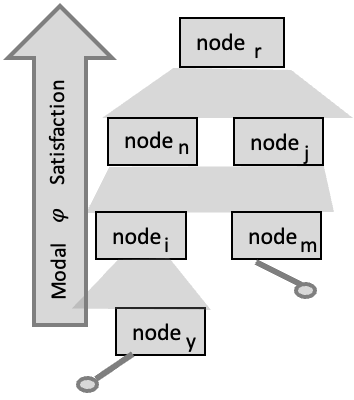
\includegraphics[width=0.25\textwidth]{entail.png}
%   \caption{Understanding the level of $\varphi$ satisfaction in the \textsc{CoW} tree of modal nodes}
%    \label{fig:nodeentail} 
% \end{wrapfigure}
% We use a modality similar to $\text{\faSitemap}@[\ell]\phi$ to indicate that $\phi$ is true of the tree node rooted at $\ell$, as well as at \emph{all reachable children} of that node.
% This means that establishing a particular $\phi$ throughout a tree must be done in a bottom-up manner (see Figure \ref{fig:nodeentail}).
% Capturing this modally, rather than with more typical ad-hoc hand-crafted invariants, offers advantages in a number of proof steps, in addition to concisely capturing intuitive reasoning about subtrees with all nodes satisfying a particular property. One basic example is that while the actual disk sync code requires the full filesystem tree to be in an amplified state (hence write amplification), most of the filesystem works with more general trees. Since $\phi_{\textsf{amplified}}\vdash\phi_{\textsf{valid}}$, using our \faSitemap modality we can conclude $\text{\faSitemap}@[\ell]\phi_{\textsf{amplified}}\vdash\text{\faSitemap}@[\ell]\phi_{\textsf{valid}}$ by an analogue of Axiom K.
% There are also other places in the code where a subtree satisfying a stronger assertion at all nodes must be linked into a larger tree satisfying only a weaker assertion overall: predicate representing the valid tree as the tree of nodes which are backed by resources allocated pages, i.e. $\phi_{\textsf{valid}}$, is weaker than the predicate representing the tree of nodes being currently amplified in the current snapshot. Again, the same reasoning principle makes this straightforward. As alluded to earlier, our $\phi_{\textsf{amplified}}$ and company are in fact \emph{predicates} parameterized by a choice of node, though by lifing \textsf{Iris}'s BI structure they can use all of the standard separation logic connectives. 
%\colinsaysinl{I cut some text here about the three-way split (commented out) that I wasn't sure how to use, but maybe I deleted something important?}
%To put it concretely, as shown in Figure \ref{fig:cow_index_tree.JPG}, \textsc{CoW} semantics determine what we can claim on the structure of the filesystem indexing tree:
%\begin{itemize}
%\item The bottom-up direction splits the tree into the two half at the cursor node: 1. the bottom part accessible from the cursor node and per-node-amplification is reflected in case needed 2. the upper part on which amplifcation has not reflected yet. 
%\item Horizontally, amplifcation path splits the bottom part of the tree into three different contexts: untouched tree nodes, nodes on the amplification path, and the ones generated as part of node splitting. 
%\end{itemize}
%Based on these two observations, in fact, bottom-up amplification determines the choice of modal context by giving the boundries of \textit{any claimable knowledge} (e.g. $\varphi_{\textsf{amplified}}$, $\varphi_{\textsf{untouched}}$): a subtree bounded by the cursor node.
%$\paragraph{Strong Nominalization} Some resource elements require strong \emph{association} with their contexts as \emph{up-to} proper identification of resource context. That means, not only does the resource context have to be identified with a nominal, but also resource elements need to be associated with some nominals that are related to the context nominal, because certain actions in operational semantics require \emph{identification} of the resource context and elements together. For a stack with $m$ regions, returning from a i$^{th}$ index roughly (ignoring the evaluation context issues related to the underlying logic):
%\[
%\infer{\textsf{wp} \; return \; cont^{i}(K') \{Q\}_n}{%
%\begin{array}{l}
%    \textsf{ExistsRegion} \; m  \quad\quad   n <= m - i  \quad\quad i <= m  \\
%\textsf{ExistsRegion} \; (m-i) -\ast \; \overset{.}{\hookrightarrow}^{m-i} (\textsf{wp} \; K'[shift \; i] \;\{Q\}_n)  \end{array}
%}
%\]
%asserting that with proper stack region lower bound (n), and the index falling to the proper range, knowing that the next required precondition ($(\textsf{wp} \; K'[shift \; i] \;\{Q\}_n)$) is independent of any stack points-to ($\fbox{m-i} \;\ell \mapsto v$) above the region $m-i$ by the StackRegion Modality (as an instance of NextGen Modality)  $\overset{.}{\hookrightarrow}^{m-i}$ (Independence Modality ~\cite{larsnextgen25}). Here, we see that both the resource context (Region Modality) and the resource elements (stack points-to assertions) nominalized, and they are aware of each other. Regarding the Post-Crash Modality, since Perennial utilizes it for extending Hoare triple encoding of Perennial with the crash recovery ( \textsf{wpc} ~\cite{tejperennial19, tejthesis}) such that in case a crash occurs on a disk-access, Hoare triple decorated with the crash recovery condition utilizes the capabilities in the crash invariant for the n$^{th}$ successful disk state (what NextGen ~\cite{larsnextgen25} calls \emph{generation} number). Since Post-Crash Modality is parameterized with the resource names ($\overline{\gamma}$), based on these resource names, the in-memory updates ($p \mapsto^{\gamma}_n v$) are ignored and only relevant successful disk updates ($d[p] \mapsto^{\gamma'}_n v$) are considered to create the consistent crash invariant n+1, $\fbox{C}_{n+1}$. Since NextGen Modality ~\cite{larsnextgen25} generalizes Perennial, lifting Post-Crash Modality into the client specification would require \emph{strong nominalization} as the proof would require the guarantees similar to the StackRegion Modality (Independence Modality ~\cite{larsnextgen25}) asserting the updates on disk are \emph{independent} of any in-memory updates.
%
%%When we look at the third column, we see the modal program logics that require strong normalization. Thinking of in-memory updates to be persistent on the disk, Perennial ~\cite{tejperennial19} decorates the in-memory ownership capabilities, which is resource elements of the  (e.g. $p \mapsto_{n} v_0$) with generation numberbrs 
%%For example, the resource elements in the separation logic utilizing \textsf{NextGen} modality and the modality itself are subject to strong normalization: both weakest-precondition and the ownership assertions are nominalized with region index such that the ownerships are valid as long as the constraint on the region index is satisfied -- e.g., all the ownership assertions with region index greater than the one on the weakest-precondition are valid against a crash-step in a filesystem or garbage collecting step in another system updating the consistent disk or reclaimed memory layout. \todo[inline]{maybe paraphrase more on referring them in the ambient logic}.
%
%\paragraph{Weak Context Nominalization} Unlike the resources we discussed so far, some resource elements are \emph{agnostic} to the resource context they belong. That means the resource context needs a nominalization as it needs to be distinguished from other resource contexts when certain actions in the operational semantics are taken (e.g., address-space switch in Table \ref{table:decomposition}), but the resource elements of the context are unaware of this context nominalization, and they may even not be labeled with any other nominal as well. For example, virtual memory references in an address space do not know which address space they belong, but the address spaces are distinguished w.r.t. the unique memory address of the root page-table tree therefore, a virtual-address-points-to ownership assertion does not need to be aware (or nominalized with) of the nominal of the address-space which is the unique memory address of the address table. Logically, specifying an address-space switch ~\cite{kuru2025modalabstractionsvirtualizingmemory} from the address space with the root address $r2$ to the one with the root address $r1$
%\[
%\{[r1] P \ast Q \} cr3 := r1 \{P \ast [r2]Q\}_{\textsf{cr3}}
%\]
%requires having the resource elements to be loaded into the memory 
%\[P \triangleq \ell_1 \mapsto v ...\]
%to be in the resource context of the address-space modality with the nominal $r1$, and, once the new address space is loaded --- i.e., cr3 is loaded with the other address-space root address ---, the resource elements ($Q$) that were loaded in the previous view of the memory are now introduced to the resource context with the nominal $r2$. Unlike what we discuss in the strong normalization (e.g. StackModality in Return specification) in which nominalized resource elements (stack points-to assertions) are guarded by Independence Modality ~\cite{larsnextgen25} (StackModality row in Table \ref{table:decomposition}) to preserve the soundness of the proof rule. However, with weak-nominalization, resource elements don't have nominals (Address-Space Modality Resource Element Column in Table \ref{table:decomposition}), and most importantly, address-space resource context switch, unlike shifted stack region in Return Specification, does not require any explicit independence check because all the resource elements at any time are either in one of two resource contexts or hosted in the ambient logic.

%\begin{definition}[Transforming Resource Context in Resource Ambience]
%    For the examples in this paper, a Resource ambiance is always a Hoare Triple indexed with the resource context nominals, which hosts the resource contexts. Unlike the transformation of resource elements hosted by a resource context (\textbf{Definition 3.3.}) handled by a relation in the modality definition, e.g. the resource element transformation relation in Post-Crash modality, updating the resource contexts themselves depends on the operational semantics action ( the last column in Table \ref{table:decomposition}) a resource ambiance is operating on.
%\end{definition}
%The address-space switch updating the cr3 register that holds the nominal value for address-space modality's resource contexts and the resource ambiance's (Hoare Triple indexed with resource context nominal) is an example of updating a resource context in a resource ambiance.
%\paragraph{Composition of Contingent Truth} Another example of weak-nominalization is Ref-Counter Modality (jump modality ($@_{l} \; P$ ~\cite{amalreal2024}) shown in Table \ref{table:decomposition}. The resource context $@_{l} \; P$ is a container of memory nodes (i.e. the resource elements ($\ell \mapsto v$ in Table \ref{table:decomposition}) that are \emph{reachable} by a jump over the shared/duplicable root address $\ell$. In addition to being weakly nominalized due to its agnostic resource elements, it exhibits a good example of how one contingent truth \emph{entails} another. Wagner et.al., also define \emph{reachability} modality --- a monad style modality for specification of non-destructive actions ($\blackdiamond$) ~\cite{amalreal2024} --- to assert the reachability to a certain memory node. Knowing $P$ satisfied under \emph{jump} ~\cite{amalreal2024} modality (\textsf{Ref-Counter Modality} in \ref{table:decomposition}) entails the satisfaction of $P$ under non-destructive reachability modality
%\[ 
%@_{\ell} \;P \vdash  \blackdiamond \; P 
%\]
%\begin{definition}[Resource Interaction]
%A resource interaction rule defines a particular way to interact with a resource context to access resource elements. A resource interaction is defined by a proof rule with the relevant resource context in the specification. 
%\end{definition}
%Although it is almost always the case that when a modality is defined, classical proof rules such as introduction and elimination are also defined and proven. However, an interesting perspective emerges when we realize that, in fact, the proof rule for switching address spaces resembles an introduction (also elimination) rule for adding resource elements into an address-space modality's resource context.
%\Colin{So far I like how this is shaping up as a kind of ``design recipe'' for approaching this style of verification!}
\textbf{Conclusion}
\label{sec:conclusion}
% \todo[inline]{this definitely needs adjusting for both audience and emphasis on this being a survey}
A systematic pattern emerging in the use of modalities in the verification of low-level systems software,
and explained how a range of modern work fits into this pattern.
So not only are the modalities observably present, but they are demonstrably useful
for conducting proofs of systems software.
%  the pieces we have identified seem to be an effective way of working out
% a specific modality for a specific use-case.
We believe that these essential patterns in the designs of modal abstractions for systems verification constitute a fundamental
concept
when working out how to specify different kinds of systems code.
\bibliographystyle{ACM-Reference-Format}
\bibliography{software}


%%
%% If your work has an appendix, this is the place to put it.
\appendix


\end{document}
\endinput
%%
%% End of file `sample-sigconf-authordraft.tex'.
